\section{Bibliographie}

\subsection{Avantage d'un système de gestion bibliographique}
\begin{slide}
  \begin{itemize}
    \item Aide à la gestion des sources.
    \item Uniformité du style de référence.
    \item Assurance de ne pas oublier une référence dans la bibliographie finale.
    \item Gestion automatique des abréviations (\emph{op. cit.}, \emph{idem.} etc).
    \item Correction rapide en cas d'erreur.
  \end{itemize}
\end{slide}
\subsection{Les types d'entrées bibliographiques}
\begin{slide}
  \begin{itemize}
    \item Nombreux types standards
      \begin{description}
	\item[basiques] article, book, proceedings, collection, reference, website etc.
	\item[avancées] mvbook, inbook, bookinbook etc.
      \end{description}
    \item Avec des packages supplémentaires : bookinarticle, manuscript etc.
    \item Possibilités de créer ses propres types. 
  \end{itemize}
\end{slide}
\subsection{Les types de champs}
\begin{slide}
  \begin{itemize}
    \item Nombreux champs standards
      \begin{description}
	\item[basiques] author, editor, title, series, journal,  publisher etc.
	\item[avancées] maintitle, pagination, shortseries,  annotator, etc.
      \end{description}
    \item Avec des packages supplémentaires : realauthor (et d'autres à l'avenir).
    \item Possibilités de créer ses propres champs.
  \end{itemize}
\end{slide}

\subsection{Le mécanisme d'héritage}

\begin{slide}
  \begin{itemize}
    \item Système de sous-entrées.
    \item Permet d'hériter des champs des entrées mères : limite le risque d'erreur.
    \item Permet de choisir à la fin de n'afficher que les entrées mères, que les entrées filles ou les deux.
\end{itemize}
\end{slide}

\begin{slide}
 \centering
 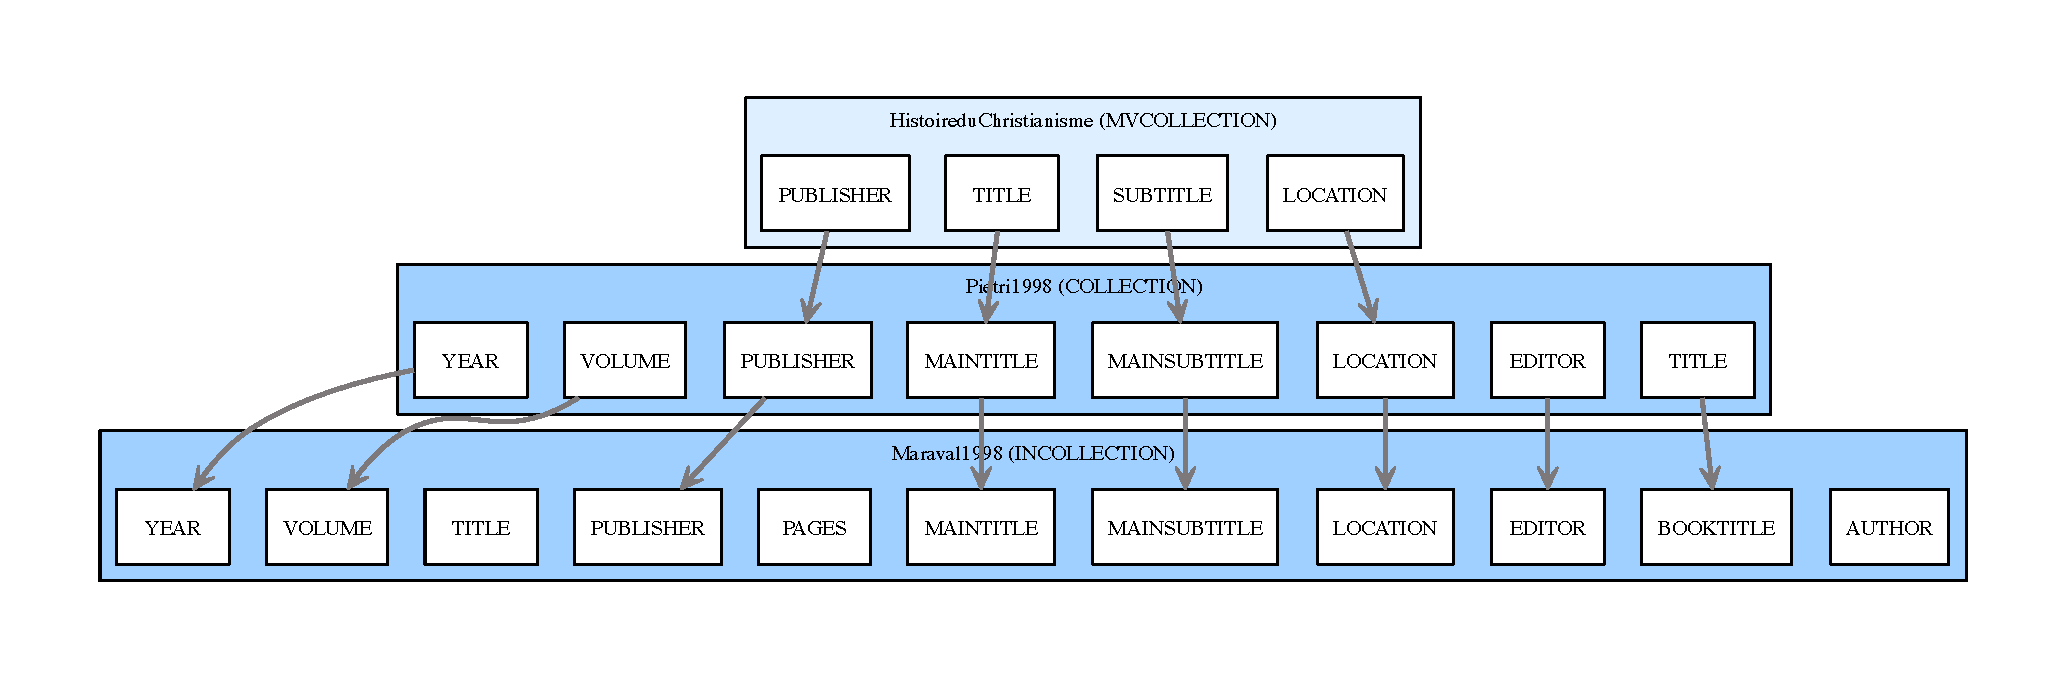
\includegraphics[width=\textwidth]{heritage.pdf}

 \cite{Maraval1998}
\end{slide}

\subsection{Système de citation}

\begin{slide}
  \begin{columns}
    \begin{column}[t]{0.45\textwidth}
      \begin{minted}{tex}
      	\footcite{BHG226}
	
	\footcite[(3)630]{Pleiade_Barnabe}

	\footcite[(1)629]{Pleiade_Barnabe}

	\footcite{BHG226}
    \end{column}

    \begin{column}
	\cite{BHG226}
	
	\cite[(3)630]{Pleiade_Barnabe}

	\cite[(1)629]{Pleiade_Barnabe}

	\cite{BHG226}

    \end{column}
  \end{columns}
\end{slide}
